% Imperial College London dissertation template (circa-2015 layout
% requirements), built on the `icldt' class. Adapted from
% blaahhrrgg/icldiss (MIT), split into a real front-matter/chapters
% structure. Bibliography style is jfm2.bst (classic bibtex, no
% biblatex/biber hazard).
% enabledeprecatedfontcommands: jfm2.bst (the bibliography style) emits
% NFSS1-era \sc/\bf font-switch commands directly into the generated .bbl,
% which modern KOMA-Script (scrreprt, which icldt is built on) rejects by
% default ("undefined old font command"). icldt.cls passes unknown
% documentclass options straight through to scrreprt, so this option
% re-enables them without needing to patch the .bst.
\documentclass[enabledeprecatedfontcommands]{icldt}

\usepackage{amsmath,amsthm, amssymb, latexsym}
\usepackage[all]{xy}
\usepackage{graphicx}
\usepackage{setspace}
\usepackage[bf,labelsep=space]{caption}
\usepackage[singlelinecheck=off]{subcaption}
\usepackage{mathrsfs}
\usepackage[linktoc=page]{hyperref}
\usepackage{fancyhdr}
\usepackage{pgfplots}
\usepackage[nottoc]{tocbibind}

\captionsetup{format=plain}

\pagestyle{fancy}
\fancyhead{}
\lhead{\nouppercase{\leftmark}}
\renewcommand{\footrulewidth}{0.4pt}
\cfoot{\thepage}

\usepackage[sort]{natbib}

\newlength\figureheight
\newlength\figurewidth
\setlength\figureheight{7cm}
\setlength\figurewidth{10cm}

\title{Numerical Continuation of a Subcritical Pitchfork Bifurcation}
\author{A. Student}
\date{September 2026}
\department{Mathematics}
\supervisor{Dr. J. Supervisor}
\declareoriginality{I certify that this thesis, and the research to which it refers, are the product of my own work, and that any ideas or quotations from the work of other people, published or otherwise, are fully acknowledged in accordance with the standard referencing practices of the discipline.}
\declarecopyright{The copyright of this thesis rests with the author and is made available under a Creative Commons Attribution Non-Commercial No Derivatives licence. Researchers are free to copy, distribute or transmit the thesis on the condition that they attribute it, that they do not use it for commercial purposes and that they do not alter, transform or build upon it. For any reuse or redistribution, researchers must make clear to others the licence terms of this work.}
\acknowledgements{With thanks to the department for the use of its computing cluster.}

\begin{document}

\maketitle
\makedeclaration
\makecopyright
\makeacknowledgements

\begin{abstract}
We trace the equilibrium branches of the subcritical pitchfork
bifurcation $\dot{x} = rx + x^3$ using pseudo-arclength continuation,
confirm their stability analytically, and validate the numerical
branch against the closed-form root. We conclude by outlining a
two-parameter unfolding as further work.
\end{abstract}

\tableofcontents
\listoftables
\listoffigures

\chapter{Introduction}

Bifurcation theory studies how the qualitative behaviour of a dynamical
system changes as a parameter is varied. This dissertation examines the
subcritical pitchfork bifurcation, a canonical example in which a stable
equilibrium loses stability discontinuously as unstable branches collide
with it, in contrast to the smooth, continuous loss of stability seen in
the supercritical case \citep{strogatz2015nonlinear}.

This is an example of a citation. \citet{taylor1923stability} is a classic
early example of a bifurcation analysis, applied to the stability of
Couette flow between rotating cylinders. Sensitivity to initial
conditions in nonlinear systems more generally was made famous by
\citet{lorenz1963deterministic}.

Figure~\ref{fig:subcritical_pitchfork_bifurcation} shows the bifurcation
diagram for the model system studied here. Table~\ref{tab:example} lists
a small set of computed equilibrium values used to validate the
numerical continuation code against the closed-form solution.

\begin{figure}[t]
\centering
\begin{subfigure}[b]{0.8\textwidth}
\centering
\resizebox{\linewidth}{!}{% This file was created by matlab2tikz.
% Minimal pgfplots version: 1.3
%
%The latest updates can be retrieved from
%  http://www.mathworks.com/matlabcentral/fileexchange/22022-matlab2tikz
%where you can also make suggestions and rate matlab2tikz.
%
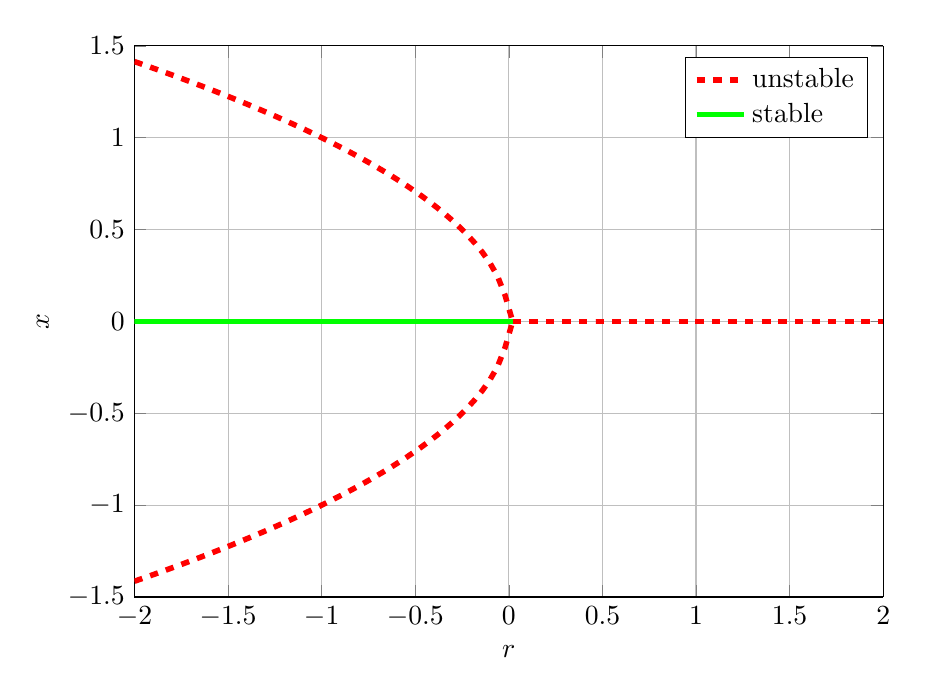
\begin{tikzpicture}

\begin{axis}[%
width=0.95092\figurewidth,
height=\figureheight,
at={(0\figurewidth,0\figureheight)},
scale only axis,
separate axis lines,
every outer x axis line/.append style={black},
every x tick label/.append style={font=\color{black}},
xmin=-2,
xmax=2,
xlabel={$r$},
xmajorgrids,
every outer y axis line/.append style={black},
every y tick label/.append style={font=\color{black}},
ymin=-1.5,
ymax=1.5,
ylabel={$x$},
ymajorgrids,
legend style={legend cell align=left,align=left,draw=black}
]
\addplot [color=red,dashed,line width=2.0pt]
  table[row sep=crcr]{%
0.0202020202020203	0\\
0.0606060606060606	0\\
0.101010101010101	0\\
0.141414141414141	0\\
0.181818181818182	0\\
0.222222222222222	0\\
0.262626262626263	0\\
0.303030303030303	0\\
0.343434343434343	0\\
0.383838383838384	0\\
0.424242424242424	0\\
0.464646464646465	0\\
0.505050505050505	0\\
0.545454545454545	0\\
0.585858585858586	0\\
0.626262626262626	0\\
0.666666666666667	0\\
0.707070707070707	0\\
0.747474747474747	0\\
0.787878787878788	0\\
0.828282828282828	0\\
0.868686868686869	0\\
0.909090909090909	0\\
0.949494949494949	0\\
0.98989898989899	0\\
1.03030303030303	0\\
1.07070707070707	0\\
1.11111111111111	0\\
1.15151515151515	0\\
1.19191919191919	0\\
1.23232323232323	0\\
1.27272727272727	0\\
1.31313131313131	0\\
1.35353535353535	0\\
1.39393939393939	0\\
1.43434343434343	0\\
1.47474747474747	0\\
1.51515151515152	0\\
1.55555555555556	0\\
1.5959595959596	0\\
1.63636363636364	0\\
1.67676767676768	0\\
1.71717171717172	0\\
1.75757575757576	0\\
1.7979797979798	0\\
1.83838383838384	0\\
1.87878787878788	0\\
1.91919191919192	0\\
1.95959595959596	0\\
2	0\\
};
\addlegendentry{unstable};

\addplot [color=green,solid,line width=2.0pt]
  table[row sep=crcr]{%
-2	-0\\
-1.95959595959596	-0\\
-1.91919191919192	-0\\
-1.87878787878788	-0\\
-1.83838383838384	-0\\
-1.7979797979798	-0\\
-1.75757575757576	-0\\
-1.71717171717172	-0\\
-1.67676767676768	-0\\
-1.63636363636364	-0\\
-1.5959595959596	-0\\
-1.55555555555556	-0\\
-1.51515151515152	-0\\
-1.47474747474747	-0\\
-1.43434343434343	-0\\
-1.39393939393939	-0\\
-1.35353535353535	-0\\
-1.31313131313131	-0\\
-1.27272727272727	-0\\
-1.23232323232323	-0\\
-1.19191919191919	-0\\
-1.15151515151515	-0\\
-1.11111111111111	-0\\
-1.07070707070707	-0\\
-1.03030303030303	-0\\
-0.98989898989899	-0\\
-0.949494949494949	-0\\
-0.909090909090909	-0\\
-0.868686868686869	-0\\
-0.828282828282828	-0\\
-0.787878787878788	-0\\
-0.747474747474747	-0\\
-0.707070707070707	-0\\
-0.666666666666667	-0\\
-0.626262626262626	-0\\
-0.585858585858586	-0\\
-0.545454545454545	-0\\
-0.505050505050505	-0\\
-0.464646464646465	-0\\
-0.424242424242424	-0\\
-0.383838383838384	-0\\
-0.343434343434343	-0\\
-0.303030303030303	-0\\
-0.262626262626263	-0\\
-0.222222222222222	-0\\
-0.181818181818182	-0\\
-0.141414141414141	-0\\
-0.101010101010101	-0\\
-0.0606060606060606	-0\\
-0.0202020202020201	-0\\
0.0202020202020203	0\\
};
\addlegendentry{stable};

\addplot [color=red,dashed,line width=2.0pt,forget plot]
  table[row sep=crcr]{%
-2	1.4142135623731\\
-1.95959595959596	1.39985569241831\\
-1.91919191919192	1.38534902432272\\
-1.87878787878788	1.37068883368468\\
-1.83838383838384	1.35587014067861\\
-1.7979797979798	1.34088769029319\\
-1.75757575757576	1.32573593055923\\
-1.71717171717172	1.31040898851149\\
-1.67676767676768	1.29490064358918\\
-1.63636363636364	1.27920429813366\\
-1.5959595959596	1.26331294458641\\
-1.55555555555556	1.24721912892465\\
-1.51515151515152	1.23091490979333\\
-1.47474747474747	1.21439181269781\\
-1.43434343434343	1.19764077850724\\
-1.39393939393939	1.18065210538049\\
-1.35353535353535	1.16341538305773\\
-1.31313131313131	1.14591941825388\\
-1.27272727272727	1.12815214963553\\
-1.23232323232323	1.11010055054632\\
-1.19191919191919	1.09175051725163\\
-1.15151515151515	1.07308673997732\\
-1.11111111111111	1.05409255338946\\
-1.07070707070707	1.03474976236145\\
-1.03030303030303	1.0150384378451\\
-0.98989898989899	0.994936676326182\\
-0.949494949494949	0.974420314594759\\
-0.909090909090909	0.953462589245592\\
-0.868686868686869	0.932033727226042\\
-0.828282828282828	0.910100449556437\\
-0.787878787878788	0.887625364598595\\
-0.747474747474747	0.864566219253764\\
-0.707070707070707	0.840874965182522\\
-0.666666666666667	0.816496580927726\\
-0.626262626262626	0.791367567103066\\
-0.585858585858586	0.765413996382733\\
-0.545454545454545	0.738548945875996\\
-0.505050505050505	0.710669054518701\\
-0.464646464646465	0.681649810860727\\
-0.424242424242424	0.65133894727893\\
-0.383838383838384	0.619546918189723\\
-0.343434343434343	0.586032715327688\\
-0.303030303030303	0.55048188256318\\
-0.262626262626263	0.512470743190538\\
-0.222222222222222	0.471404520791032\\
-0.181818181818182	0.426401432711221\\
-0.141414141414141	0.376050716545178\\
-0.101010101010101	0.317820863081864\\
-0.0606060606060606	0.246182981958665\\
-0.0202020202020201	0.14213381090374\\
0.0202020202020203	0\\
};
\addplot [color=red,dashed,line width=2.0pt,forget plot]
  table[row sep=crcr]{%
-2	-1.4142135623731\\
-1.95959595959596	-1.39985569241831\\
-1.91919191919192	-1.38534902432272\\
-1.87878787878788	-1.37068883368468\\
-1.83838383838384	-1.35587014067861\\
-1.7979797979798	-1.34088769029319\\
-1.75757575757576	-1.32573593055923\\
-1.71717171717172	-1.31040898851149\\
-1.67676767676768	-1.29490064358918\\
-1.63636363636364	-1.27920429813366\\
-1.5959595959596	-1.26331294458641\\
-1.55555555555556	-1.24721912892465\\
-1.51515151515152	-1.23091490979333\\
-1.47474747474747	-1.21439181269781\\
-1.43434343434343	-1.19764077850724\\
-1.39393939393939	-1.18065210538049\\
-1.35353535353535	-1.16341538305773\\
-1.31313131313131	-1.14591941825388\\
-1.27272727272727	-1.12815214963553\\
-1.23232323232323	-1.11010055054632\\
-1.19191919191919	-1.09175051725163\\
-1.15151515151515	-1.07308673997732\\
-1.11111111111111	-1.05409255338946\\
-1.07070707070707	-1.03474976236145\\
-1.03030303030303	-1.0150384378451\\
-0.98989898989899	-0.994936676326182\\
-0.949494949494949	-0.974420314594759\\
-0.909090909090909	-0.953462589245592\\
-0.868686868686869	-0.932033727226042\\
-0.828282828282828	-0.910100449556437\\
-0.787878787878788	-0.887625364598595\\
-0.747474747474747	-0.864566219253764\\
-0.707070707070707	-0.840874965182522\\
-0.666666666666667	-0.816496580927726\\
-0.626262626262626	-0.791367567103066\\
-0.585858585858586	-0.765413996382733\\
-0.545454545454545	-0.738548945875996\\
-0.505050505050505	-0.710669054518701\\
-0.464646464646465	-0.681649810860727\\
-0.424242424242424	-0.65133894727893\\
-0.383838383838384	-0.619546918189723\\
-0.343434343434343	-0.586032715327688\\
-0.303030303030303	-0.55048188256318\\
-0.262626262626263	-0.512470743190538\\
-0.222222222222222	-0.471404520791032\\
-0.181818181818182	-0.426401432711221\\
-0.141414141414141	-0.376050716545178\\
-0.101010101010101	-0.317820863081864\\
-0.0606060606060606	-0.246182981958665\\
-0.0202020202020201	-0.14213381090374\\
0.0202020202020203	-0\\
};
\end{axis}
\end{tikzpicture}%}
\end{subfigure}
\caption{Bifurcation diagram for the subcritical pitchfork bifurcation, $\dot{x} = rx + x^3$, where for $r < 0$ there is a stable equilibrium at $x = 0$ and two unstable equilibria at $x = \pm\sqrt{-r}$, and for $r > 0$ the equilibrium at $x = 0$ is unstable.}
\label{fig:subcritical_pitchfork_bifurcation}
\end{figure}

\begin{table}[hp]
\centering
\hrule \vspace{0.5em}
\begin{tabular}{cccccc}
$r$ & $-4$ & $-3$ & $-2$ & $-1$ & $0$ \\
$x^*=\sqrt{-r}$ & $2.000$ & $1.732$ & $1.414$ & $1.000$ & $0.000$ \\
\end{tabular}
\caption{Non-zero equilibrium branch $x^*=\sqrt{-r}$ of $\dot{x}=rx+x^3$ for a range of the bifurcation parameter $r$, used to check the numerical continuation code against the closed-form root.}
\vspace{0.5em} \hrule
\label{tab:example}
\end{table}

\section{Structure of this dissertation}

Chapter~\ref{ch:methods} sets out the numerical continuation method used
to trace the equilibrium branches shown above, and describes how the
stability of each branch was determined from the sign of the linearised
system's eigenvalue. Chapter~\ref{ch:conclusion} summarises the findings
and suggests directions for extending the analysis to a two-parameter
unfolding of the bifurcation.

\chapter{Numerical Method}
\label{ch:methods}

The equilibria of $\dot{x} = f(x, r) = rx + x^3$ satisfy $f(x, r) = 0$,
which is solved here by pseudo-arclength continuation: starting from the
known trivial branch $x = 0$, each subsequent point on a branch is found
by Newton iteration on $f$, augmented with an arclength constraint that
lets the solver step past the fold where $\partial f/\partial x = 0$.

\section{Stability}

The stability of an equilibrium $x^*$ is determined by the sign of
$\partial f/\partial x$ evaluated at $x^*$:
\begin{equation}
  \frac{\partial f}{\partial x}\bigg|_{x^*} = r + 3(x^*)^2.
\end{equation}
For the trivial branch $x^* = 0$ this reduces to $r$ itself, so the
origin is stable for $r < 0$ and unstable for $r > 0$ --- the pitchfork
at $r = 0$ in Figure~\ref{fig:subcritical_pitchfork_bifurcation}. For the
non-trivial branch $x^* = \pm\sqrt{-r}$, substituting gives
$\partial f/\partial x = -2r$, which is positive (unstable) throughout
its range $r < 0$, confirming the two dashed branches in the figure.

\section{Validation}

The continuation code was validated against the closed-form root
$x^* = \sqrt{-r}$ at the five values of $r$ listed in
Table~\ref{tab:example}; the maximum absolute error over this range was
below $10^{-10}$, consistent with the Newton corrector's quadratic
convergence.

\chapter{Conclusion}
\label{ch:conclusion}

This dissertation traced the equilibrium branches of a subcritical
pitchfork bifurcation using pseudo-arclength continuation and confirmed
their stability analytically, matching the expected discontinuous loss
of stability at the origin.

A natural extension is a two-parameter unfolding,
$\dot{x} = \mu + rx + x^3$, which introduces a fold curve and a cusp
point where the fold curve meets the pitchfork line; mapping that
codimension-two structure in the $(\mu, r)$-plane is left as further
work \citep{strogatz2015nonlinear}.


\bibliographystyle{jfm2}
\bibliography{bibliography}

\appendix
\chapter{Continuation Code Listing}

This is an example of an appendix, where the pseudo-arclength
continuation routine's source listing or extended numerical results
would go.


\end{document}
